\chapter{Verfahren zur Echtzeit Optimierung von Augmented Reality durch Tiefeninformationen}

Anhand der Klassifizierung von Project Tango bezüglich Augmented Reality aus Abschnitt \ref{sec:classification_project_tango}, kann bereits festgehalten werden, dass sich das Gerät, durch die Verfügbarkeit von intrinsischen und extrinsischen Kameraparametern, für den Einsatz von Augmented Reality gut eignet. \\ 

Um jedoch eine optimierte Augmented Reality Anwendung umsetzen zu können, benötigt man laut \citet{azuma2001recent} die Möglichkeit mehr Informationen über relevante Objekte im reellen Raum zu ermitteln. Diese Informationen könnten zum Beispiel eine Tiefenüberdeckung von virtuellen Objekten durch reale Objekte ermöglichen. Eine weitere Idee ist die Interaktion mit realen Objekten durch die Anwendung von physikalischen Modellen und Kollisionen. Die Information, auf die sich hier fokussiert werden sollen sind die Tiefeninformationen, die Project Tango durch Depth Perception in Form einer Pointcloud liefern kann.\\

Die folgenden Abschnitte widmen sich mit den Verfahren zur möglichen Realisierung dieser Optimierungen durch Tiefeninformationen. Das Erste Verfahren ermöglicht eine Überdeckung virtueller Objekte durch Depth Maps. Hiernach werden zwei existierende Verfahren zur Echtzeit Rekonstruktion näher behandelt. Zuletzt werden verschiedene Algorithmen zu einer Echtzeit planaren Rekonstruktion kombiniert und näher erläutert. \\

\section{Verdeckung durch Depth Maps}

\section{Echtzeit Polygon Rekonstruktion} \label{sec:polygon_reconstruction}

Die Idee der Verdeckung mit Hilfe des Z-Buffers lässt sich nicht nur mit Depth Maps realisieren. Auch Primitiven oder allgemein Polygone könnten mit Hilfe eines entsprechenden Fragment Shaders, als Repräsentation der Umgebung, andere virtuelle Objekte Transparent überlagern, um die Illusion der Überdeckung von realen Objekten zu ermöglichen. Somit ließe sich das Problem der Optimierung von Augmented Reality mit Hilfe von Tiefeninformation auf das Echtzeit Rekonstruktions Problem zurückführen. \\

Die 3D Rekonstruktion ist bereits ein etabliert Forschungsgebiet in der Computer Grafik und gewinnt, auf Grund von kostengünstigen Consumer Tiefensensoren, wie die Microsoft Kinect, Asus Xtion oder Structure \citep{Struc48:online}, zunehmend an Bedeutung. Dabei wird sich immer mehr auf die Echtzeit Rekonstruktion konzentriert, da diese Geräte in der Lage sind, Tiefeninformationen, zwar mit leichten Messfehlern aber in Echtzeit, zu liefern. \citet{niessner2013real} erwähnen an dieser Stelle zudem den möglichen Einsatz für Augmented Reality:

\begin{quote}
\enquote{The ability to obtain reconstructions
in real-time opens up various interactive applications including:
augmented reality (AR) where real-world geometry can be fused
with 3D graphics and rendered live to the user; ...} \citep{niessner2013real}
\end{quote}

Die Herausforderung in der Echtzeit Rekonstruktion liegt dabei in der möglichst performanten Fusion von mehreren überlagernden Depth Maps. Hieraus soll eine möglichst detailierte Repräsentation der echten Umgebung generiert werden, welche sich im Idealfall stetig verbessert. Diese Problemstellung unterscheidet sich von herkömmlichen Rekonstruktionsverfahren wie die von \citet{hoppe1992surface} und der Poission Rekonstruktion von \citet{kazhdan2006poisson}. Aktuelle Verfahren nutzen dafür verschiedenste optimierte Datenstrukturen, welche zudem durch den Einsatz von entsprechenden GPU Implementierungen beschleunigt werden können. Dennoch spielt die Gegenüberstellung von Detailgrad, der Skalierung und Geschwindigkeit stets eine große Rolle. \citet{niessner2013real} \\

Bekannte Verfahren wie KinectFusion \citep{newcombe2011kinectfusion}, ein SLAM Verfahren von \citet{bylow2013real} oder DynamicFusion \citep{newcombe2015dynamicfusion} nutzen Truncated Signed Distance Function, kurz TSDF, zur Speicherung und Migration der Oberflächeninformation mehrerer Depth Maps. Das Verfahren von \citet{niessner2013real} erweitert diesen Ansatz mit einem effizienten Spartial Hashing Verfahren, um die Zugriffszeiten und Speicherverbrauch zu minimieren. Darüber hinaus nimmt das Verfahren Chisel von \citep{Klingensmith_2015_7924} diese Vorzüge auf und kombiniert TSDF mit  \enquote{visual-inertial odometry}, der Trackingtechnologie von Project Tango. In den folgenden Absätzen werden die Mechanismen hinter TSDF, dem räumlichen Hashing näher Erläutert. Hiernach soll auch noch auf das Rendering der TSDF Oberfläche durch Marching Cubes und auf die weiteren Optimierungen von Chisel eingegangen werden. \\


\subsection{Truncated Signed Distance Function}

Bei der von \citet{curless1996volumetric} vorgestellten räumlichen Repräsentation von Oberflächen, Truncated Signed Distance Function (TSDF), wird der Raum in Voxel einer gewünschten Auflösung unterteilt. Anders als Occupancy Maps, in denen die Voxel als sichtbar oder unsichtbar markiert werden, werden bei TSDF in den Voxeln die jeweiligen Entfernungen zur nächsten Oberfläche angegeben. Wichtig dabei ist das Vorzeichen, welches angibt, ob sich ein Voxel innerhalb oder außerhalb eines Objektes befindet.  \citep{curless1996volumetric} \\

Gefüllt wird die Repräsentation durch die Depth Maps und der entsprechenden Kameraposition, die im Fall von Project Tango bereits gegeben ist. So wird für jede Tiefeninformation ein Strahl ausgehend von der Kameraposition generiert, der die durchschnittenen Voxel aktualisiert. Der Stahl ist dabei von der Länge begrenzt, um die zu aktualisierenden Voxel zu minimieren und zudem keine Oberflächen zu aktualisieren, die sich weiter hinter der gefundenen Oberfläche befindet. Dieses Vorgehen ist in Abbildung \ref{fig:tsdf} c) zu erkennen. \citep{Compu66:online} \\

\begin{figure}
  \centering
	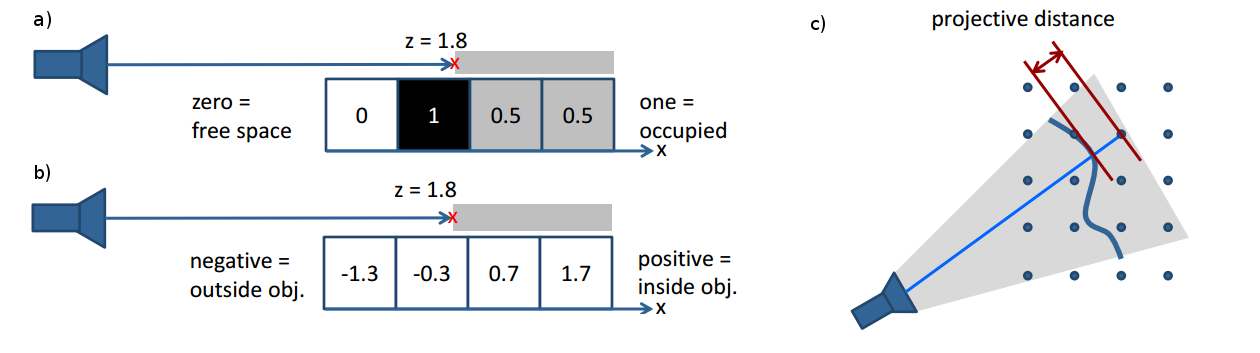
\includegraphics[width=1.0\textwidth]{content/images/methods/tsdf.png} 
  \caption{a) Beispielhafte Voxel Füllung von Occupancy Maps; b) Beispielhafte Voxel Füllung durch TSDF; c) Exemplarische 2D Darstellung der Oberfläche mit entsprechenden Strahlensatz für die TSDF. Übernommen von \citet{Compu66:online}}
  \label{fig:tsdf}
\end{figure}

Der Vorteil dieser Repräsentation liegt darin, dass die konkreten Oberflächeninformationen, anders als bei der Diskretisierung von Occupancy Maps, nicht verloren gehen. Das heißt, dass trotz einer gröberen Voxel Struktur stets der Nulldurchgang rekonstruiert werden kann. Neben der Entfernung zur nächsten Oberfläche wird zusätzlich noch ein Gewichtungswert in jedem Voxel gespeichert. Das ermöglicht es leichtes Rauschen durch einfache Mittelung zu unterdrücken und die Oberfläche optimiert sich somit bei jeder Aktualisierung der Voxel. \citep{Compu66:online}\\

\subsection{Spartial Hashing}

Das Problem der Echtzeit Rekonstruktion ist wie bereits angesprochen die Aushandlung von Detailgrad, Skalierung der zu rekonstruierenden Szene und Performance der Rekonstruktion. Auch die TSDF Repräsentation ist sehr speicherintensiv und benötigt für die zu scannende Szene reservierten Speicher, der auf mobilen Endgeräten nur begrenzt verfügbar ist. Daher muss auch für größere Rekonstruktionen oder Rekonstruktionen unbekannter Größe ein dynamischer Ansatz gefunden werden. \citet{Klingensmith_2015_7924} erwähnt dazu, dass einige Verfahren OctTrees einsetzen, die zwar äußerst dynamisch sind, jedoch einen deutlichen Nachteil hinsichtlich der Zugriffszeiten auf die Voxel bringen. \\

\begin{figure}
  \centering
	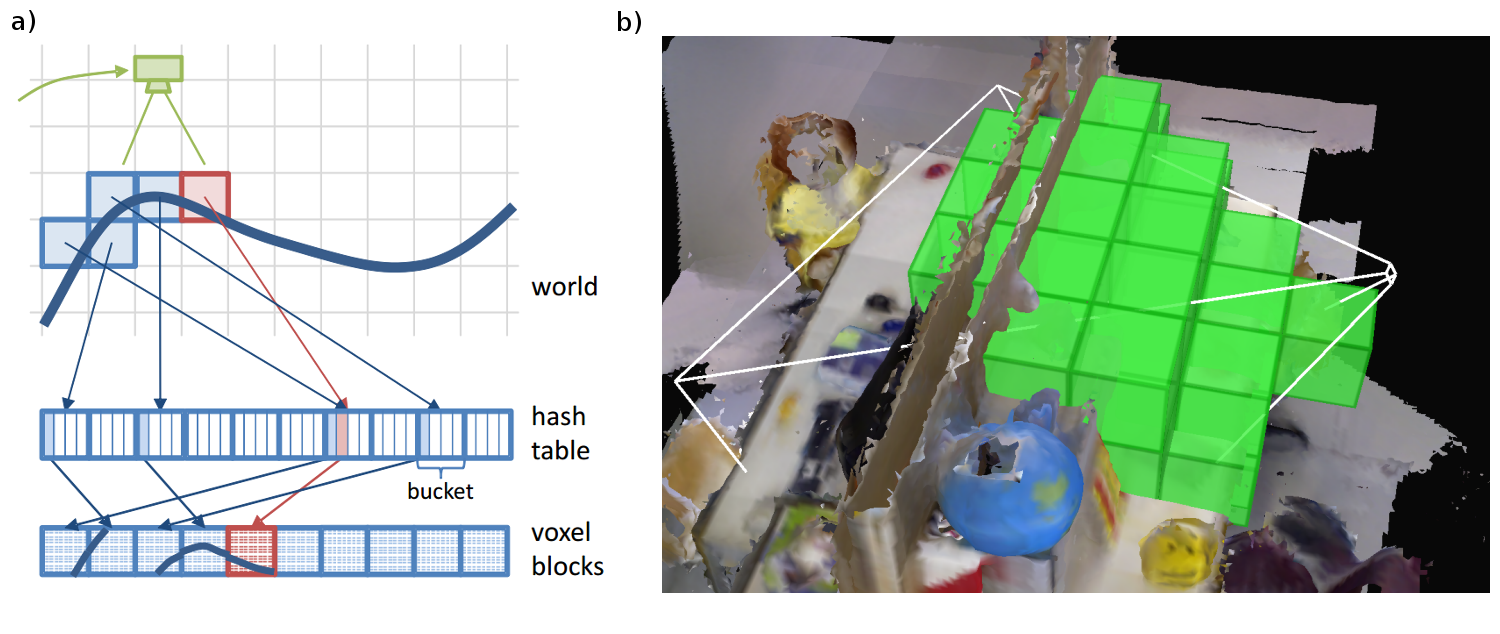
\includegraphics[width=1.0\textwidth]{content/images/methods/hashing.png} 
  \caption{a) Voxel Hashing Datenstruktur. Übernommen von \citet{niessner2013real} b) Darstellung der relevanten Voxel Chunks für die Aktualisierung. Übernommen von \citet{Klingensmith_2015_7924}}
  \label{fig:hashing}
\end{figure}

\citet{niessner2013real} führen daher eine zwei-Ebenen Baumstruktur ein, die auf der zweiten Ebene als Menge von Voxel räumlich zusammenfassen. Diese werden hier Chunks genannt. Auf der ersten Ebene können diese Chunks in einer Hash Tabelle räumlich mit einer Hashfunktion identifiziert werden. Das ermöglicht somit einen nahezu direkten Zugriff auf räumliche Voxel und ermöglicht es zudem Chunks dynamisch allokieren. Als Hash der Chunkposition \(x\), \(y\) und \(z\) wird die folgende Hashfunktion aus Gleichung \ref{eq:spatial_hash} verwendet. Bei den Variablen \(p_1\), \(p_2\) und \(p_3\) handelt es sich um willkürlich hohe Primzahlen und \(n\) entspricht der Größe der Hash Tabelle.

\begin{equation}\label{eq:spatial_hash}
H(x,y,z) = (x * p_1 \oplus y * p_2 \oplus z * p_3) \mod n
\end{equation}

\subsection{Marching Cubes}

Die meisten Echtzeit Rekonstruktionen durch TSDF wie KinectFusion sind GPU Umsetzungen, die daher die Möglichkeit besitzen ein hardwarebeschleunigtes Rendering durch Raycasting durchzuführen. Das Verfahren Chisel von \citet{Klingensmith_2015_7924} nutzt hingegen einen indirekten Weg zum Rendering durch die Marching Cubes Triangulation. \\

\begin{figure}
  \centering
	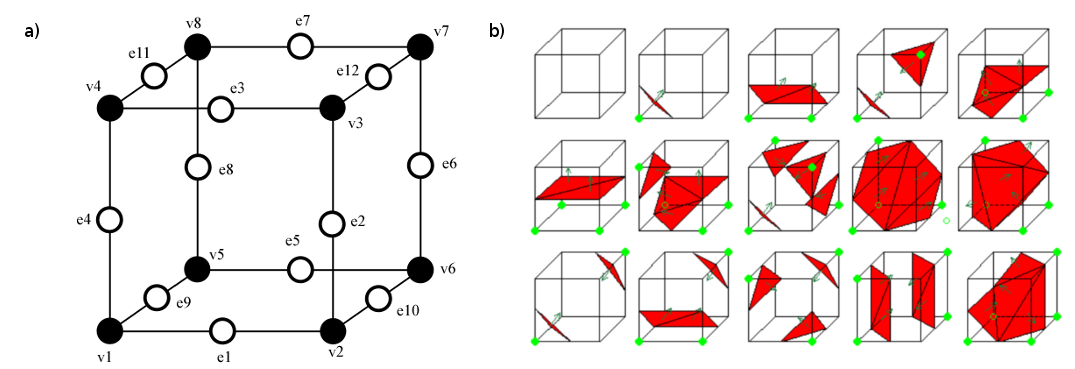
\includegraphics[width=1.0\textwidth]{content/images/methods/marchingcubes.png} 
  \caption{a) Marching Cubes Voxel Repräsentation mit den Ecken und den Kantenschnittpunkten b) Die 15 möglichen 3D Polygon Varianten. Übernommen von \citet{MarchingCubes:online}}
  \label{fig:marchingcubes}
\end{figure}

Marching Cubes nach \citet{lorensen1987marching} ist ein Algorithmus um aus einer als Voxel repräsentierten Isofläche Polygone zu bestimmen, die diese Fläche möglichst nah repräsentieren. Hierzu werden zu jedem Voxel die Ecken \(v1\) bis \(v8\) untersucht, ob sie innerhalb oder außerhalb eines Objektes liegen. Zusätzlich werden zu jeder Kante auf dem Voxel, wenn ein Schnitt der Isofläche existiert, die Schnittpunkte \(e1\) bis \(e12\) durch Diese bestimmt. Abbildung \ref{fig:marchingcubes} a) zeigt die Ecken und Kantenschnittpunkte eines Voxels. \\

Je nach binärer Gewichtung der Ecken können hiernach aus einem Katalog von 256 Varianten die Polygone nachgeschlagen werden. Inhalt des Katalogs sind die Indizes der Kantenschnittpunkte, aus denen Polygone generiert werden können. Alle diese 256 Varianten können auf 15 verschiedene Fälle zurückgeführt werden, die sich nur in Rotation oder Symmetrie unterscheiden. Die 15 Varianten sind in Abbildung \ref{fig:marchingcubes} b) zu finden. \citep{MarchingCubes:online} \\

\subsection{Chisel mit Space Carving}

Das Bereits erwähnte Verfahren Chisel von \citet{Klingensmith_2015_7924} verwendet alle zuvor erwähnten Techniken der TSDF, spartial Hashing und der Marching Cubes Überführung. Sie sprechen dabei von einem \enquote{dynamic spatial-hashed truncated distance field}. Das für den mobilen Einsatz optimierte Verfahren ist in der Lage eine Echtzeitrekonstruktion von Räumen von bis zu \(300 m^2\) mit einem Detailgrad von zwei bis drei Zentimetern zu erstellen. Zudem können neben Tiefeninformationen auch gefärbte Pointclouds verarbeitet werden, wodurch ein gefärbtes Mesh generiert werden kann. \citep{Klingensmith_2015_7924}\\

\begin{lstlisting}[mathescape,caption=Chisel TSDF Algorithmus, label=lst:chisel]
Eingabe: Pointcloud $C$, Kameratransformation $P_{cam}$, 
         Strahlenbegrenzung $t$

für jeden Tiefenwert $\vec{p}$ aus $C$
    bestimme die Oberflächenposition $\vec{z}$ aus $\vec{p}$ und $P_{cam}$
    bestimme einen Strahl $\vec{r}$ aus $\vec{z}$ und $P_{cam}$
    bestimme den Begrenzungsbereich $t_{vor}$, $t_{nach}$ mit $t$ um $\vec{z}$ auf $\vec{r}$
    # space carving
    für jeden Voxel $v$ zwischen Kamera und $t_{vor}$
        wenn die Distanz im Voxel negativ ist
            setze Voxel zurück
    # normale TSDF Bestimmung
    für jeden Voxel $v$ zwischen $t_{vor}$ und $t_{nach}$
        bestimme die Voxeldistanz zu $z$
        setze das Gewicht w des Voxels $v$
\end{lstlisting}

Zusätzlich erweitern sie den TSDF Algorithmus um die \enquote{space carving} Funktionalität. Sie betrachten dabei den Strahl von der Kamera zur Oberfläche als eine Art Constraint, in dem alle durchstoßenden Voxel bis zur Oberfläche eine negativen Wert beinhalten müssen. Ist das nicht der Fall, so wird ein Voxel außerhalb der inneren Begrenzung auf den leeren Ursprungswert gesetzt. Im Pseudocode aus Listing \ref{lst:chisel} wird das Verhalten näher erläutert. Diese Verbesserung führt dazu, dass die Rekonstruktion bei stark rauschenden Tiefeninformationen, besonders an Objektkanten, deutlich verbessert wird. Außerdem ist das Verfahren hiermit in der Lage dynamische Änderungen in der Umgebung zu detektieren und neue Oberflächen entsprechend zu aktualisieren. So beeinflussen, zum Beispiel, sich im Bild bewegen Personen nur kurz die TSDF. \citep{Klingensmith_2015_7924}\\

Neben space carving wurden zudem eine variable Strahlenbegrenzungen und Gewichtungen der Voxel abhänig von der jeweils aufgenommenen Tiefe implementiert. Diese Funktion berücksichtigt die Verteilung von Messungenauigkeiten des Sensors, die bei größerer Entfernung der Oberfläche zum Tiefensonsor zunehmen können. \citep{Klingensmith_2015_7924}

\section{Planare Rekonstruktion}

Wie bereits in Absatz \ref{sec:polygon_reconstruction} beschrieben, lässt sich das Problem der Optimierung von Augmented Reality mit Hilfe von Tiefeninformationen auf eine Echtzeit Rekonstruktion zurückführen. Im Gegensatz zur Rekonstruktion komplexer Oberflächen, mit dem vorgestellten TSDF Verfahren, soll hier eine Idee näher erläutert werden, die eine Rekonstruktion allein auf planaren Primitiven ermöglicht. \citet{yang2010plane} erwähnt hierzu, dass Ebenen in fast allen künstlichen Umgebungen zu finden sind und auf Grund ihrer vorteilhaften geometrischen Eingenschaften in verschiedensten Computer Vision Verfahren verwendet werden. Daher gibt es viele Forschungsarbeiten, Methoden und Algorithmen um aus verschiedensten Informationsquellen ein Ebenenmodell zu extrahieren.\\

Wie in dem \enquote{Simultaneous Localization and Mapping} (SLAM) Verfahren von \citet{trevor2012planar} wird hier zunächst eine Ebene in der Pointcloud mit Hilfe des RANSAC Algorithmus gesucht. RANSAC bietet gegenüber anderen Algorithmen zur Ebenen Detektion den Vorteil, ein Modell auch bei vielen Ausreißern performant zu ermitteln. Agglomeratives Clustering und Region Growing wie von \citet{feng2014fast} beschreiben, eignet sich auf Grund des Ausgabeformats aus Project Tango nicht, da es keine organisierte Point Cloud ausgibt. \\

Die Repräsentation der Ebene \(P\) wird, angelehnt an das Vorgehen von \citet{trevor2012planar}, wie in Gleichung \ref{eq:plane} festgehalten. Dabei handelt es sich um den Normalenvektor \(\vec{n}\) und der Distanz zum Ursprung \(d\) der Hesse Normalform einer Ebene, sowie der Punkte der konvexen Hülle \(H\). Um die konvexe Hülle der Ebene zu bestimmen, wird der Graham Scan Algorithmus verwendet. Wie auch von \citet{trevor2012planar} beschreiben wird die konvexe in der Repräsentation festgehalten, um eine sukzessive Verbesserung einer Ebene nach mehreren Messdurchläufen zu ermöglichen. So werden die Punkte der konvexen Hülle pro Messvorgang kombiniert, damit die Ebenenausbreitung auch außerhalb des Sichtfeldes beibehalten werden kann.

\begin{equation} \label{eq:plane}
P=\left[\vec{n}, d, H\right] \qquad H=\vec{h_1}, \vec{h_2}, \ldots  \vec{h_n}
\end{equation}

Um wiederum aus dieser Repräsentation eine Triangulation zu erhalten, wird hier die zweidimensionale Sweep-Line Delaunay Triangulation durchgeführt. Die Schritte aus dem Algorithmus \ref{lst:planeReconstruction} werden in den folgenden Kapiteln näher beschreiben.

\begin{lstlisting}[mathescape,caption=Algorthmus der planaren Echtzeit Rekonstruktion, label=lst:planeReconstruction]

Eingabe: Octtree $O$
Ausgabe: Polygonpunkte $T_{Gesamt}$

für jedes Cluster $C$ aus $O$
    bestimme Ebene [$\vec{n}$, $d$, $P$] mit RANSAC aus $C_{Punkte}$
    wenn keine Ebene mit genügend $P$ in $C_{Punkte}$ gefunden wurde
    		nächstes Cluster (continue)
    wenn Ebene mit [$\vec{n}$, $d$, $H_{alt}$] in $C_{Ebenen}$ existiert	
        füge die konvexe Hülle $H_{alt}$ zu $P$ hinzu	
    bestimme die konvexe Hülle $H_{neu}$
    bestimme die Tringulation $T_{Ebene}$ aus $H_{neu}$
    $T_{Gesamt}$ += $T_{Ebene}$
    $C_{Ebenen}$ += [$\vec{n}$, $d$, $H_{neu}$]
    $C_{Punkte}$ - $P$
		

\end{lstlisting}

\subsection{RANSAC zur Ebenendetektion}

Der \enquote{RAndom SAmple Consensus} Algorithmus (RANSAC), vorgestellt von \citet{fischler1981random}, ist in der Lage, aus einer Menge von Daten mit vielen Ausreißern, die Parameter für ein passendes Modell zu schätzen. Anders als andere Schätzverfahren wie \enquote{Least-Median} oder \enquote{M-Schätzer}, welche aus der Statistik Literatur entnommen und entsprechend angepasst wurden, wurde RANSAC speziell für die Anwendung in der Computer Graphik entwickelt. Der Kern dieses Algorithmus ist das wiederholte Bestimmen eines Modells aus zufälligen und für das Modell ausreichenden Stichproben. Listing \ref{lst:ransac} zeigt den Verlauf des RANSAC Algorithmus. Die Anzahl der Iterationen \(N\) hängt dabei allein von dem Anteil der Ausreißer in den Messwerten ab. Daher sollte sie entsprechend gewählt werden, um die Wahrscheinlichkeit zu verringern, dass Ausreißer in den Stichproben enthalten sind. \citep{derpanis2010overview} \\

\begin{lstlisting}[mathescape,caption=Der RANSAC Algorithmus, label=lst:ransac]
Eingabe: Messwerte $P$, Modelltoleranz $e$, maximale Iterationen $N$
Ausgabe: Modell $m$, Unterstützende Messwerte $P_m$

1. Wähle zufällig so viele Stichproben aus den Messwerten $P$,
   wie nötig sind, um das Modell zu bestimmen
2. Bestimme aus den gewählten Stichproben das Modell $m$
3. Ermittle die Anzahl der Messwerte $P$, die mit einer 
   entsprechenden Toleranz $e$ das ermittelte Modell $m$ 
   unterstützen
4. Wenn prozentual genügend Messwerte aus $P$ das Modell $m$ 
   unterstützen, ermittle aus den unterstützenden Messwerten 
   $P_m$ durch lineare Regression erneut das finale Modell 
   $m$ und terminiere
5. Wiederhole die Schritte 1-4 $N$ mal
\end{lstlisting} 

Um mit dem RANSAC Algorithmus Ebenen in einer Punktewolke bestimmen zu können, werden pro Iteration drei Stichproben \(A\), \(B\) und \(C\) gewählt. Das Ebenenmodell, hier in der Hesse Normalform mit dem Normalenvektor \(\vec{n}\) und dem Abstand zum Koordinatenursprung \(d\), lässt sich dabei durch die Gleichung \ref{eq:normalform} bestimmen.

\begin{equation}\label{eq:normalform}
\vec{n} =\left|\left| \vec{AB} \times \vec{AC}\right|\right|
\qquad
\vec{D} = \vec{A} \cdot \vec{n}
\qquad
d = D_1 + D_2 + D_3
\end{equation}

Um zu ermitteln ob ein Punkt \(P\) aus einer Messreihe die gefundene Ebene \(\left[\vec{n_E}, d_E\right]\) unterstützt, wird die kürzeste Distanz \(d_P\) zwischen Punkt und Ebene wie in Gleichung \ref{eq:plane-distance} ermittelt.  Ein entsprechender Toleranzwert für die Distanz \(d_{min}\), im gezeigten RANSAC Algorithmus \(e\) genannt, wird später bei der Umsetzung abhängig vom Rauschen des Tiefensensors gewählt. 

\begin{equation} \label{eq:plane-distance}
d_P = n_1*P_1+n_2*P_2+n_3*P_3-d_E \qquad support_{d_P} = d_P < d_{min}
\end{equation}

Um das finale Modell der Ebene zu ermitteln, und somit die Varianz des Abstands der Punkte zur Ebene zu minimieren, wird mit Hilfe der unterstützenden Punkte \(P_{support}=\left[x,y,z\right]\) eine lineare Regression durchgeführt. Diese Mittelt ein Ebenenmodell \(E=\left[a,b,c\right]\) aus den zuvor ermittelten Punkten mit Hilfe des \enquote{least squares} Schätzverfahren. Für eine Ebene versucht man die Funktion \(G(a,b,c)\) aus Gleichung \ref{eq:least-squares} zu minimieren. Hierzu muss das lineare Gleichungssystem in Gleichung \ref{eq:least-squares-solution}  gelöst werden. \citep{Regre94:online}

\begin{equation} \label{eq:least-squares}
z = ax + by + c   \qquad G(a, b, c) = \sum {\left(z_i - ax_i - by_i - c\right)}^2
\end{equation}

\begin{equation} \label{eq:least-squares-solution}
\begin{bmatrix}
\sum x_i^2 & \sum x_iy_i & \sum x_i\\ 
\sum x_iy_i  & \sum y_i^2  & \sum y_i \\ 
\sum x_i & \sum y_i  & n
\end{bmatrix}
*
\begin{bmatrix}
a\\ 
b\\ 
c
\end{bmatrix}
=
\begin{bmatrix}
\sum x_iz_i\\ 
\sum y_iz_i\\ 
\sum z_i
\end{bmatrix}
\end{equation}

\subsection{Bestimmung der Ebenenausbreitung}

Nachdem die Ebene und die korrespondierenden Punkte zur Ebene gefunden wurden, muss noch die Ausbreitung der Fläche bestimmt werden, da die Ebene in Hesse Normalform lediglich die Position \(\vec{n} * d\) und Ausrichtung \(\vec{n}\) festhält. \citet{PlanarSurfaceMapping} nutzt hierfür die konvexe Hülle der korrespondierenden Punkte und trianguliert diese. Um das performant umzusetzen, kann man sich hier die Eigenschaft der Ebene zu Nutzen machen und die dreidimensionalen Punkte durch Parallelprojektion als zweidimensionale Punkte auf die Ebene projizieren. Denn die Algorithmen für die Triangulation haben im zweidimensionalen eine deutlich besseres Laufzeitverhalten. \\

Nach der Triangulation können die Ecken der gefundenen Polygone jeweils zurück projiziert werden. Die Gleichungen \ref{eq:projection2d} und \ref{eq:projection3d} bilden die Projektion der Punkte wobei \(R_{\vec{n}to\vec{z}}\) der Rotationsmatrix zwischen dem Normalenvektor \(\vec{n}\) und der Z-Achse \(\vec{z}\) entspricht.\\

\begin{equation} \label{eq:projection2d}
p_{2d} = (p_{3d} - (\vec{n}*d)) * R_{\vec{n}to\vec{z}}
\end{equation}
\begin{equation} \label{eq:projection3d}
p_{3d} = (p_{2d} * R_{\vec{n}to\vec{z}}^{-1}) + (\vec{n}*d)
\end{equation}

\subsubsection{Convex Hull Algorithmus}

Für die Berechnung der konvexen Hülle wird der Graham Scan nach \citet{graham1972efficient} genutzt. Dieser Algorithmus besitzt eine Laufzeit von \(O(n \log n)\) und gilt als einer der populärsten Algorithmen für die Berechnung der konvexen Hülle. Andere Ansätze besitzen dabei ein ähnliches oder schlechteres Laufzeitverhalten. Gestartet wird der Algorithmus mit der Menge aller Punkte \(P\) der Ebene und mit einem Startpunkt \(P_0\), der Bestandteil der konvexen Hülle ist. Hierzu wird meist der Punkt mit dem niedrigsten \(y\) Faktor gewählt. (\(P_0=P_{min(y)}\)) Listing \ref{lst:graham-scan} zeigt den Verlauf des Algorithmus des Graham Scans. Dabei wird in Abbildung \ref{fig:convexhull} nochmals die erste Sortierung und das Unterscheidungskriterium für die Sortierung als auch für die Aussortierung der Punkte verdeutlicht. \citep{convexHull} \\

\begin{figure}
  \centering
	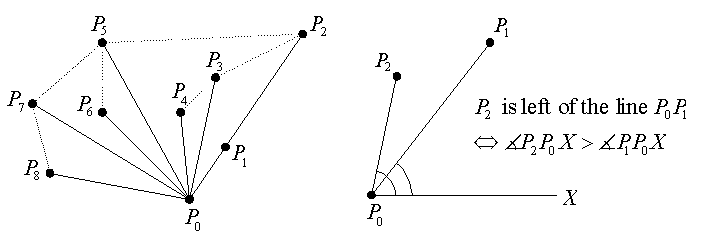
\includegraphics[width=0.9\textwidth]{content/images/methods/convexhull.png} 
  \caption{Sortierung der Punkte nach Winkel zum Startpunkt (links) mit dem Unterscheidungskriterium (rechts). Übernommen von \citet{convexHull}}
  \label{fig:convexhull}
\end{figure}

\begin{lstlisting}[mathescape,caption=Graham Scan Algorithmus, label=lst:graham-scan]
Eingabe: Menge der Punkte $P$, außen liegender Punkt $P_0$
Ausgabe: Punkte der konvexen Hülle

$i$ = 0
sortiere nach dem Winkel zu $P_0$
solange $i$ <= $|P|$
    wenn $\measuredangle P_{i-1} P_{i}$ > $\measuredangle P_{i-1} P_{i+1}$, also $P_i$ rechts von  $\vec{P_{i-1} P_{i+1}}$ liegt
        inkrementiere $i$
    ansonsten
        entferne $P_i$ aus $P$
        dekrementiere $i$
    
\end{lstlisting} 


\subsubsection{Triangulation}

Nachdem die konvexe Hülle bestimmt wurde, müssen die Punkte dieses Pfades noch trianguliert werden. Hierfür wird eine Delaunay-Triangulation mit Hilfe des Sweep-Line Algorithmus von \citet{domiter2008sweep} verwendet. Unter einer Delaunay-Triangulation versteht man zunächst einmal eine Art Constraint, der sogenannten Umkreisbedingung, die besagt, dass ein Kreis, der alle drei Punkte eines gefundenen Polygons durchzieht, keine weiteren Punkte beinhalten darf. \\

Nähere Beschreibung des Algorithmus ...

\subsection{Planare Rekonstruktion als Echtzeit Umsetzung}

\subsubsection{Clusteringverfahren}

